
Varjo ei välttämättä ole aina avautumisen jälkeen täysin kehittynyt vaan vaatii kierteiden poiston ja/tai pumppausta (\ref{hyppytapahtuma-varjon-avautuminen-ja-lentokuntoon-saattaminen} s.\pageref{hyppytapahtuma-varjon-avautuminen-ja-lentokuntoon-saattaminen}). Molemmat ovat aivan normaaleja toimenpiteitä varsinkin pakkolaukaisuhypyillä (syynä esimerkiksi huono uloshyppy tai lentokoneen alhainen ilmanopeus). Varjo lentää, vaikka punoksissa on kierrettä, kuvun reunatunnelit ovat tukossa ja slider on ylhäällä, mikäli varjo täyttää lentävän laskuvarjon kriteerit: 

\begin{framed}
\begin{itemize}
\item  Kupu on säännöllisen muotoinen. 
\item  Punokset ovat kireällä. 
\item  Slider on suorakaiteen muotoinen. 
\end{itemize}
\end{framed}

Muista aina tarkkailla korkeutta, jotta voit tarvittaessa ajoissa suorittaa varavarjotoimenpiteet. 


\textbf{Jos et osaa päättää, lentääkö päävarjo vai ei, se EI LENNÄ!} => Tee varavarjotoimenpiteet! 

\section{ Lentää, Täysin kehittynyt }
\label{paavarjon-vajaatoiminnot-lentaa-taysin-kehittynyt}


\begin{Figure}\centering\includegraphics[width=0.95\textwidth]{Vajaatoiminnot-Lentaa-Taysin-kehittynyt.png}\end{Figure} 

\begin{itemize}
\item  Kupu on säännöllisen muotoinen 
\item  Punokset ovat kireällä 
\item  Slider on suorakaiteen muotoinen ja alhaalla. 
\end{itemize}

\section{ Lentää - Selvitä }
\label{paavarjon-vajaatoiminnot-lentaa-selvita}

\subsubsection{Slider ylhäällä}
\label{paavarjon-vajaatoiminnot-slider-ylhaalla}


\begin{Figure}\centering\includegraphics[width=0.95\textwidth]{Vajaatoiminnot-Lentaa-Slider-ylhaalla.png}\end{Figure} 

\begin{itemize}
\item  Pumppaa slider alas 
\item  Tarkkaile korkeutta. 
\end{itemize}
\subsubsection{Slider ylhäällä ja kierrettä}
\label{paavarjon-vajaatoiminnot-slider-ylhaalla-ja-kierretta}


\begin{Figure}\centering\includegraphics[width=0.95\textwidth]{Vajaatoiminnot-Lentaa-Slider-ylhaalla-ja-Kierteita.png}\end{Figure} 

\begin{itemize}
\item  Levitä kantohihnoja, potki kierre auki ja pumppaa slider alas 
\item  Tarkkaile korkeutta. 
\end{itemize}
\subsubsection{Reunatunnelit tukossa ja slider ylhäällä}
\label{paavarjon-vajaatoiminnot-reunatunnelit-tukossa-ja-slider-ylhaalla}


\begin{Figure}\centering\includegraphics[width=0.95\textwidth]{Vajaatoiminnot-Lentaa-Reunatunnelit-tukossa-ja-slider-ylhaalla.png}\end{Figure} 

\begin{itemize}
\item  Pumppaa slider alas ja tunnelit auki 
\item  Tarkkaile korkeutta. 
\end{itemize}
\subsubsection{Reunatunneli tukossa, slider ylhäällä ja kierrettä punoksissa}
\label{paavarjon-vajaatoiminnot-reunatunneli-tukossa-slider-ylhaalla-ja-kierretta-punoksissa}


\begin{Figure}\centering\includegraphics[width=0.95\textwidth]{Vajaatoiminnot-Lentaa-Reunatunnelit-tukossa-ja-slider-ylhaalla-ja-kierteita.png}\end{Figure} 

\begin{itemize}
\item  Levitä kantohihnoja, potki kierre auki, pumppaa slider alas ja tunneli auki 
\item  Tarkkaile korkeutta. 
\end{itemize}
\subsubsection{Avautumassa oleva varjo}
\label{paavarjon-vajaatoiminnot-avautumassa-oleva-varjo}


\begin{Figure}\centering\includegraphics[width=0.95\textwidth]{Vajaatoiminnot-lentaa-avautumassa.png}\end{Figure} 

\begin{itemize}
\item  Pumppaa kupu tarvittaessa auki 
\item  Tarkkaile korkeutta. 
\end{itemize}
\section{ Ei lennä }
\label{paavarjon-vajaatoiminnot-ei-lenna}

\subsubsection{Line over}
\label{paavarjon-vajaatoiminnot-line-over}


\begin{Figure}\centering\includegraphics[width=0.95\textwidth]{Vajaatoiminnot-line-over.png}\end{Figure} 

\begin{itemize}
\item  Tee varavarjotoimenpiteet. 
\end{itemize}

\begin{figure*}[]\centering\includegraphics[width=0.8\textwidth]{VV-toimenpiteet.pdf}\caption{VV-toimenpiteet}\end{figure*} 

\begin{verbatim} 
\end{verbatim}
\section{ Varavarjon käyttö }
\label{paavarjon-vajaatoiminnot-varavarjon-kaytto}


Tärkeät korkeudet: 

\begin{description}
\item[ 600 m ] \hfill \\ 
	\begin{itemize}
	\item  Tähän asti voit selvittää päävarjoa eli poistaa kierteitä, pumpata slideriä alas ja reunatunneleita auki. 
	\item  Jos yritykset eivät onnistu 600 metriin mennessä, tee varavarjotoimenpiteet. 
	\end{itemize}
\item[ 300 m ] \hfill \\ 
	\begin{itemize}
	\item  Tämän korkeuden alapuolella ei suositella päävarjon irtipäästöä (esimerkiksi törmättyäsi toiseen hyppääjään (\ref{mahdolliset-vaaratilanteet-tormaaminen-varjon-varassa} s.\pageref{mahdolliset-vaaratilanteet-tormaaminen-varjon-varassa})), sillä varavarjo ei välttämättä ehdi avautua. Mikäli joudut tilanteeseen, jossa sinulla on korkeutta alle 300 metriä ja päävarjosi ei lennä, avaa suoraan varavarjo tekemättä päävarjon irtipäästöä (kohdat 6-9 alla). 
	\end{itemize}
\end{description}
\subsubsection{ Varavarjotoimenpiteet }
\label{paavarjon-vajaatoiminnot-varavarjotoimenpiteet}

\begin{enumerate}[label=\bfseries \arabic*)]
\item  Pidä taivutus. 
\item  Tarkasta korkeus. 
\item  Katso päävarjon irtipäästöpampulaa (oikealla) ja ota siitä kiinni molemmin käsin. 
\item  Murra tarra ja vedä kädet suoriksi alaviistoon.  
\item  Päästä pampulasta irti 
\item  Katso varavarjon kahvaa (vasemmalla) ja ota siitä kiinni molemmin käsin. 
\item  Murra tarra ja vedä kädet suoriksi alaviistoon. 
\item  Taivuta. 
\item  Pidä vv-kahva kädessä tai päästä irti (kerhokohtainen) 
\end{enumerate}

\begin{figure*}[]\centering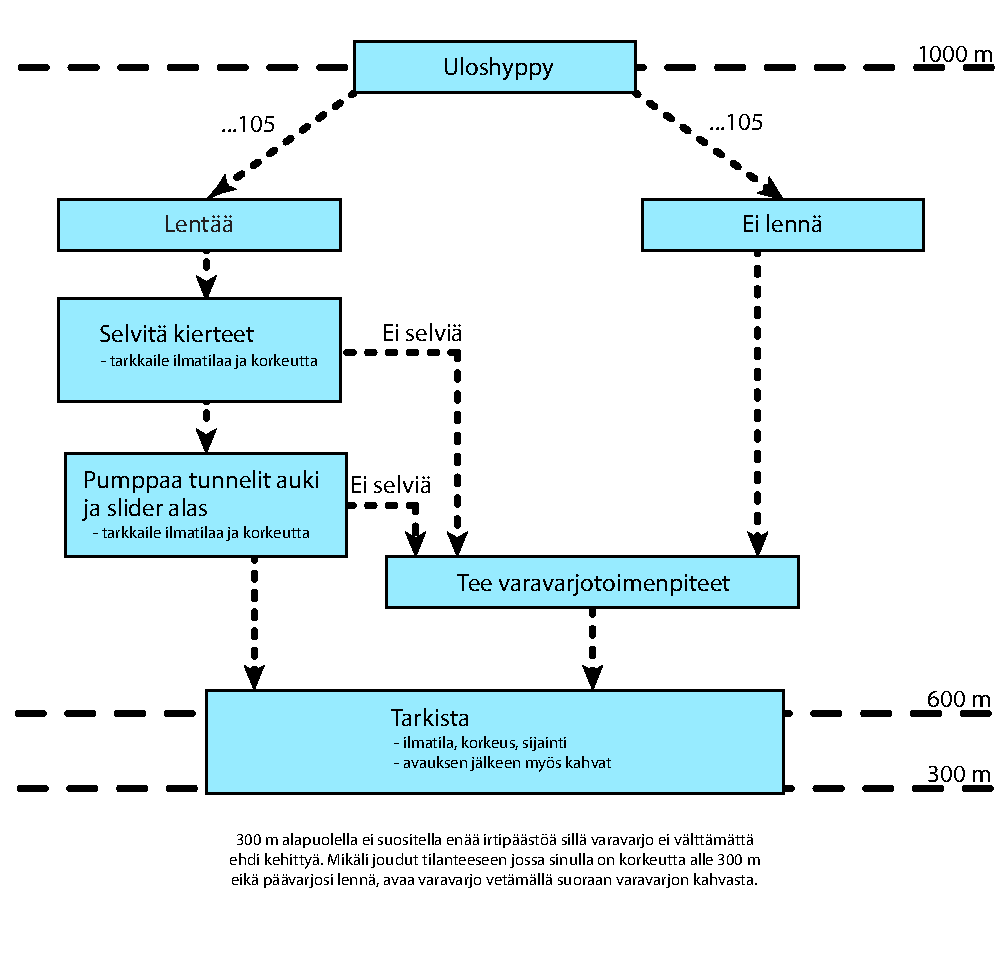
\includegraphics[width=0.99\textwidth]{VVkaavio.pdf}\caption{Toiminta päävarjon vajaatoiminnoissa}\end{figure*} 

